% Options for packages loaded elsewhere
\PassOptionsToPackage{unicode}{hyperref}
\PassOptionsToPackage{hyphens}{url}
\documentclass[
  10pt,
  letterpaper]{article}
\usepackage{xcolor}
\usepackage{amsmath,amssymb}
\setcounter{secnumdepth}{-\maxdimen} % remove section numbering
\usepackage{iftex}
\ifPDFTeX
  \usepackage[T1]{fontenc}
  \usepackage[utf8]{inputenc}
  \usepackage{textcomp} % provide euro and other symbols
\else % if luatex or xetex
  \usepackage{unicode-math} % this also loads fontspec
  \defaultfontfeatures{Scale=MatchLowercase}
  \defaultfontfeatures[\rmfamily]{Ligatures=TeX,Scale=1}
\fi
\usepackage{lmodern}
\ifPDFTeX\else
  % xetex/luatex font selection
\fi
% Use upquote if available, for straight quotes in verbatim environments
\IfFileExists{upquote.sty}{\usepackage{upquote}}{}
\IfFileExists{microtype.sty}{% use microtype if available
  \usepackage[]{microtype}
  \UseMicrotypeSet[protrusion]{basicmath} % disable protrusion for tt fonts
}{}
\makeatletter
\@ifundefined{KOMAClassName}{% if non-KOMA class
  \IfFileExists{parskip.sty}{%
    \usepackage{parskip}
  }{% else
    \setlength{\parindent}{0pt}
    \setlength{\parskip}{6pt plus 2pt minus 1pt}}
}{% if KOMA class
  \KOMAoptions{parskip=half}}
\makeatother
\usepackage{longtable,booktabs,array}
\usepackage{calc} % for calculating minipage widths
% Correct order of tables after \paragraph or \subparagraph
\usepackage{etoolbox}
\makeatletter
\patchcmd\longtable{\par}{\if@noskipsec\mbox{}\fi\par}{}{}
\makeatother
% Allow footnotes in longtable head/foot
\IfFileExists{footnotehyper.sty}{\usepackage{footnotehyper}}{\usepackage{footnote}}
\makesavenoteenv{longtable}
\usepackage{graphicx}
\makeatletter
\newsavebox\pandoc@box
\newcommand*\pandocbounded[1]{% scales image to fit in text height/width
  \sbox\pandoc@box{#1}%
  \Gscale@div\@tempa{\textheight}{\dimexpr\ht\pandoc@box+\dp\pandoc@box\relax}%
  \Gscale@div\@tempb{\linewidth}{\wd\pandoc@box}%
  \ifdim\@tempb\p@<\@tempa\p@\let\@tempa\@tempb\fi% select the smaller of both
  \ifdim\@tempa\p@<\p@\scalebox{\@tempa}{\usebox\pandoc@box}%
  \else\usebox{\pandoc@box}%
  \fi%
}
% Set default figure placement to htbp
\def\fps@figure{htbp}
\makeatother
\setlength{\emergencystretch}{3em} % prevent overfull lines
\providecommand{\tightlist}{%
  \setlength{\itemsep}{0pt}\setlength{\parskip}{0pt}}
\usepackage[]{biblatex}
\addbibresource{references.bib}
\usepackage{placeins}
\usepackage[final]{cogsci_template/cogsci}
\usepackage{float}
\usepackage{booktabs}
\setlength{\bibhang}{.125in}
% Only the corresponding author should include an email address.
\author[1]{\mbox{Marius Mercier (mariusmercier1@gmail.com)}}
\author[2]{\mbox{Ruby de Lanerolle}}
\affil[1]{IJN}
\affil[2]{UCL}

\usepackage{bookmark}
\IfFileExists{xurl.sty}{\usepackage{xurl}}{} % add URL line breaks if available
\urlstyle{same}
\hypersetup{
  pdftitle={Result reports of `Inferring Competence on a Numerical Task'},
  hidelinks,
  pdfcreator={LaTeX via pandoc}}

\title{Result reports of `Inferring Competence on a Numerical Task'}
\author{}
\date{\vspace{-2.5em}2026-01-15}

\begin{document}
\maketitle
\begin{abstract}
This is a short placeholder abstract for the CogSci submission. It will be
replaced with the final study summary once results are finalized.

\textbf{Keywords:} numerical competence; Bayesian inference; judgment; decision making
\end{abstract}

All linear Mixed Models (LMM) were computed with the ``lmerTest'' package to obtain p-values via Satterthwaite's degrees of freedom method (Kuznetsova et al., 2017). For other tests, the R packages used will be specified. For all statistical tests, alpha = 0.05.

\subsection{Behavioural Results - Manipulation Checks and Confirmatory Analysis}\label{behavioural-results---manipulation-checks-and-confirmatory-analysis}

All hypotheses and manipulation checks were supported by the participant data and the model comparisons.

Participants, given a single piece of information that another person got a particular arithmetic question right/wrong, were far better than chance at judging which other questions that person would have got right. This inference about the competence of others from very limited information relies on the participants assuming that performance on the arithmetic questions is nested, with people who can answer harder questions also being able to answer easier ones, but not vice-versa. In order to make use of the nestnessness of the questions, participants additionally needed to accurately assess the the rarity of reaching a correct answer in the time limit for different questions, in other words the difficulty of the questions. Our findings suggest that participants were on average able to make all of these judgments, enabling their successful competence inferences.

The arithmetic questions were manipulated to be nested by varying their difficulty. To verify that this manipulation resulted in nestedness of participant performance, two nestedness measures, NODF and Temperature, were calculated from a binary matrix of participants' successes/failures on each question. Each metric was computed using the oecosimu() function in the vegan package in R (Oksanen et al.~2013). The observed nestedness values (NODF or Temperature) were compared to a simulated distribution of possible values under the null hypothesis that the arithmetic questions were not nested. A higher, positive NODF indicates greater nestedness, while a lower, negative Temperature indicates greater nestedness. The primary manipulation check (\textbf{MC1}) was confirmed for both measures, with a significantly higher NODF and lower Temperature than under the null model (NODF: Z = 20.29, p = .002; Temperature: Z = -12.67, p = .002). This confirmed that participants who succeeded on hard questions (rarely answered correctly) also tended to succeed on easier ones (more commonly answered correctly). A secondary manipulation check (\textbf{MC1'}), directly derived from nesting, was then performed to check that, on average, the more difficult the question the higher the average performance score of those who got it right. Fitting a linear model with average performance score as the predictor and objective question difficulty (the rarity of answering correctly within the time limit) as the outcome, the secondary manipulation check was supported as the estimate was significantly positive (\(\beta\) = 0.24, t(13) = 13, p = \textless{} .001, Adjusted \(R^2\) = 0.92).

As a pre-requisite for the participants making use of the nested nature of the questions to infer which questions the virtual agent got right, they must be able to judge the difficulty of the questions. More specifically, they must be able to accurately assess the rarity of reaching an accurate answer within the time-limit for different questions. This was our first hypothesis (\textbf{H1}). We fit a linear mixed effects model predicting true question difficulty (the inverse of the true percentage of people who could answer correctly on the arithmetic test) with participants' perception of the question difficulty (the inverse of the percentage of people they predict could answer correctly) as the fixed effect, and random effects for participants. Confirming \textbf{H1}, the fixed effect estimate for perceived difficulty was significantly positive (\(\beta\) = 0.45, t(911.69) = 22.18, p = \textless{} .001). The high correlation between perceived difficulty and true difficultyis visible in Figure \ref{fig:S1-fig-behav}A.

\begin{figure}
\centering
\pandocbounded{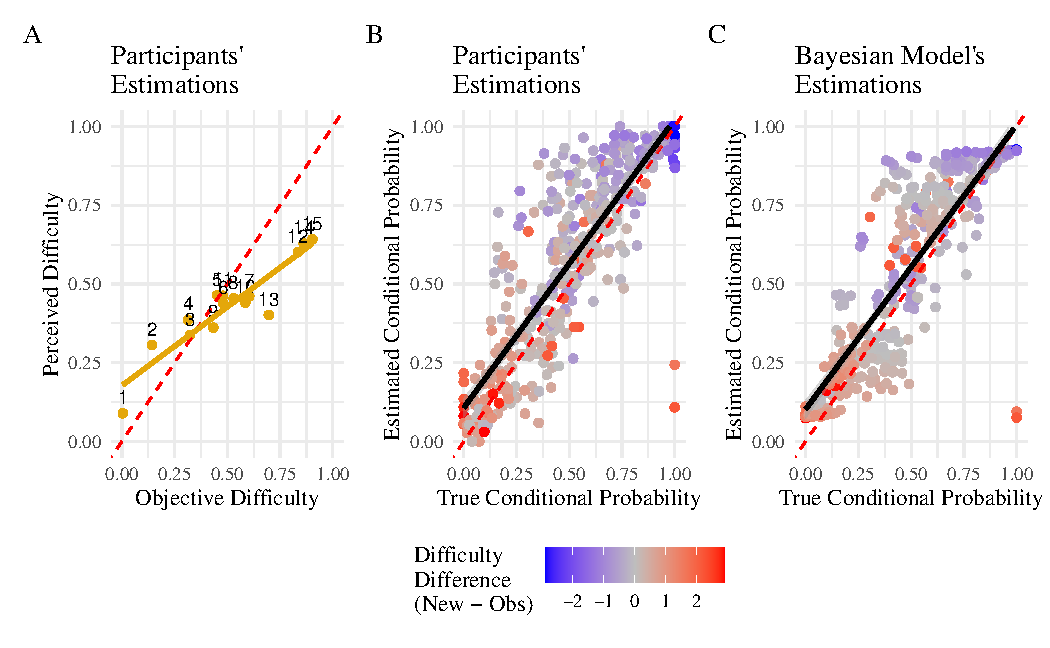
\includegraphics[keepaspectratio]{figures/S1-fig-behav-1.pdf}}
\caption{\label{fig:S1-fig-behav}\textbf{A}: Perceived Difficulty versus Objective Difficulty. Numbers refer to the question ID (see Materials). The red dashed line represents the optimal estimation. \textbf{B}: Estimated Conditional Probability versus True Conditional Probability. Each data point is a pair of two questions. The red line represents the optimal prediction while the dark line represents the fit of the linear model. \textbf{C}: Conditional robabilities estmiated by the Main Model vs True Conditional Probability. Each data point is a pair of two questions. The red line represents the optimal prediction while the dark line represents the fit of the linear model.}
\end{figure}

Participants were able to use their accurate judgments of question difficulty to then infer the arithmetic competence of another based on the observation of their success or failure on just one specific question. We aggregated their judgments of which questions would be answered correctly, conditional on success or failure on the observed question. These are the estimated conditional probability values. Then, from the participants' answers to the arithmetic questions, we computed the True Conditional Probability of answering a new question given another question was successfully answered. Our second hypothesis (\textbf{H2}) was that, on average, participants' estimations of the probabilities of success for different questions, given the observation of success/failure on a particular question, would be significantly correlated with true conditional probabilities. A linear model with the average estimated conditional probability as an dependent variable and the true conditional probability as the independent variable and confirmed participants were able to predict the true conditional probability with a great precision (\(\beta\) = 0.86, t(418) = 34.72, p \textless{} .001, Adjusted \(R^2\) = 0.74). The strong correlation between average estimated conditional probability and true conditional probability is visualized in Figure \ref{fig:S1-fig-behav}B.

We also found that participants did not have to be arithmetically competent themselves to make reasonable inferences about the competence of others. We tested whether the 30\% of participants who performed worst on the arithmetic test could still judge the difficulty of the questions (\textbf{H1m}) and whether they could accurately infer the conditional probability of answering a new question given an observed question and outcome (\textbf{H2m}). Confirming H1m with a linear mixed effect model, we found that the worst performers' perception of question difficulty was highly correlated with objective question difficulty, just as much as the for the full set of participants (\(\beta\) = 0.93, t(303) = 44.51, p \textless{} .001).

Confirming H2m with a linear model, we found that the worst performers' were still very accurate in predicting which other questions the virtual agent would succeed at, with a high correlation between true and judged conditional probabilities (\(\beta\) = 0.85, t(448) = 34.03, p \textless{} .001, Adjusted \(R^2\) = 0.72).

\subsection{Modelling Results - Confirmatory Analyses}\label{modelling-results---confirmatory-analyses}

To interrogate the predictive power of our the Bayesian Model, we tested three main hypotheses: (\textbf{H3}) posited that the predictions of the Main Model would be positively correlated with participants' average predictions. In addition, we hypothesized that, when fitted to the aggregated dataset, the Main Model would better capture participants' behavior than the Threshold heuristic model (\textbf{H4}) and the Anchor heuristic model (\textbf{H5}).

For each model, we determined the optimal free parameters by maximizing the log-likelihood of participants' responses, given the specific model and its parameter set.

\[
\mathcal{L}(\mathcal{M}_1 \mid x) = \sum_{i=1}^{N} y_i \log  P(p(x_i)) + (1 - y_i) \log (1- p(x_i))
\]

In the Main model, we varied the prior mean (\(\mu\)) between 0 and 1, the standard deviation (\(\sigma\)) between 0.05 and 1, the noise parameter between 0.05 and 1, and the beta parameter of the softmax function between 0 and 10. In the Threshold heuristic model, only the beta parameter was varied. In the Anchor heuristic model, both the beta parameter and the difficulty parameter were adjusted. All models received the following inputs: the fact that the virtual agent succeeded (\(S = 1\)) on a question with perceived difficulty \(D_{\text{obs}}\), and a request to predict the likelihood of success on a new question with perceived difficulty \(D_{\text{new}}\). Table \ref{tab:S1-table} indicates the best fitting parameters for each model.

Investigating \textbf{H3}, we fit three linear models to compare the Main Model's and the two heuristic models' fit with participants' answers, as well as how much variance in participant behaviour they explained. We found that our Main Model was very strongly correlated with participant behaviour (\(\beta\) = 0.94, t(418) = 58.29, p \textless{} .001, Adjusted \(R^2\) = 0.89). The Threshold model showed lower correlation with the data (\(\beta\) = 0.63, t(418) = 16.4, p \textless{} .001, Adjusted \(R^2\) = 0.39). The Anchor model was the weakest fit to the data (\(\beta\) = 0.77, t(418) = 24.39, p \textless{} .001, Adjusted \(R^2\) = 0.59). Figure \ref{fig:S1-fig-model-comparison} shows participants' average prediction for each possible pair of arithmetic questions (observed and judged) compared to the three models' predictions.

\begin{figure}
\centering
\pandocbounded{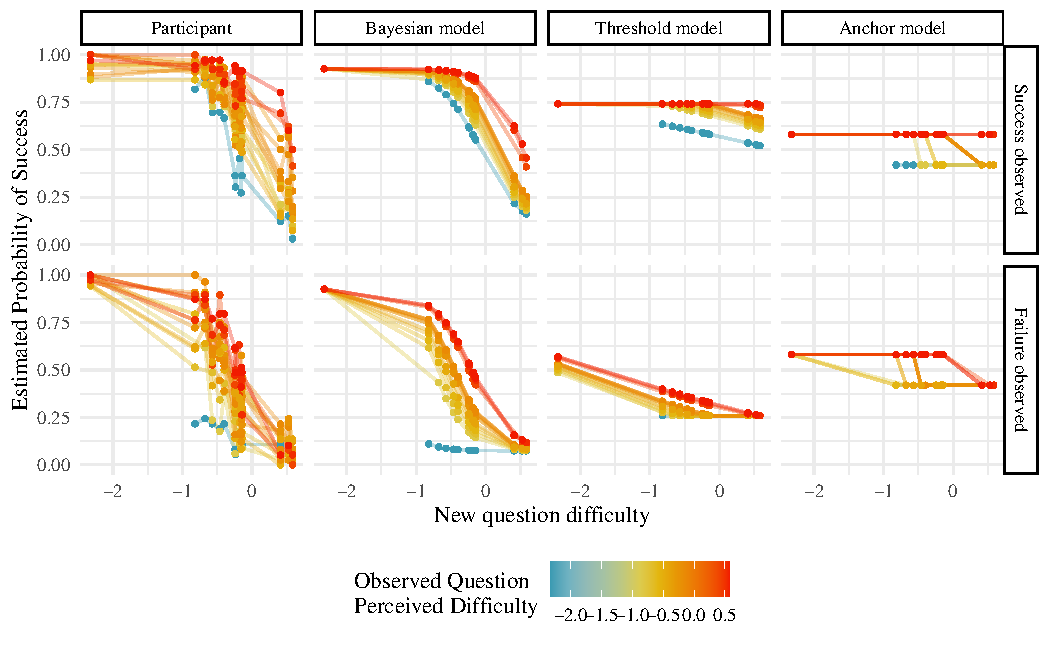
\includegraphics[keepaspectratio]{figures/S1-fig-model-comparison-1.pdf}}
\caption{\label{fig:S1-fig-model-comparison}Model comparison. Each data point is a pair of two questions.}
\end{figure}

To test \textbf{H4} and \textbf{H5}, we computed the Bayesian information criterion (BIC) using the maximum log-likelihood for each fitted model, which applies a penalty for model complexity. The Main Model, when fitted to the complete dataset, outperformed both alternative models (\(BIC_{Bayes}\) = \ensuremath{1.6063719\times 10^{4}}; \(BIC_{Threshold}\) = \ensuremath{1.9411919\times 10^{4}}; \(BIC_{Anchor}\) = \ensuremath{1.8259962\times 10^{4}}), confirming \textbf{H4} and \textbf{H5} respectively. The difference between the BIC of the Main Model and that of the next best heuristic model (Anchor Model) was 2196.2432309, which indicates very strong evidence in favor of our Main Model according to the standard interpretation criteria (Raftery, 1995).

\begin{table*}

\caption{\label{tab:S1-table}Optimised Parameters for Bayesian, Threshold and Anchor Models}
\centering
\begin{tabular}[t]{lllllllll}
\toprule
Type of Fit & Model & LLmax & BIC & \$\textbackslash{}mu\$ & \$\textbackslash{}sigma\textasciicircum{}2\$ & \$\textbackslash{}varepsilon\$ & \$\textbackslash{}Delta\$ & \$\textbackslash{}beta\$\\
\midrule
Same parameters for all participants & Bayes & -8012 & 16064 & -0.07 & 0.55 & 0.43 &  & 2.53\\
Same parameters for all participants & Threshold & -9701 & 19412 &  &  &  &  & 1.05\\
Same parameters for all participants & Anchor & -9120 & 18260 &  &  &  & 0.33 & 1.11\\
Participant-specific parameters & Bayes & -26.7 (10.19) & 70.66 (20.38) & 0.07 (1.33) & 0.78 (0.68) & 0.91 (0.87) &  & 5.91 (3.06)\\
Participant-specific parameters & Threshold & -41.83 (8.9) & 87.97 (17.81) &  &  &  &  & 1.22 (0.85)\\
\addlinespace
Participant-specific parameters & Anchor & -36.11 (9.9) & 80.86 (19.8) &  &  &  & 0.78 (0.77) & 1.47 (0.73)\\
\bottomrule
\multicolumn{9}{l}{\rule{0pt}{1em}\textit{Note: }}\\
\multicolumn{9}{l}{\rule{0pt}{1em}We use the same parameters for all participants in the Average Model Comparison and we use participant-specific parameters for the Exploratory Analyses. For participant-specific parameters, we report the average inferred parameters along with the standard deviation in parenthesis.}\\
\end{tabular}
\end{table*}

\subsection{Exploratory Analysis}\label{exploratory-analysis}

As further exploratory analysis, we investigated several research questions. The first was whether if we divide the data by whether the participants observed a virtual agent's success or failure, participants' mean predictions of the probabilities of success still correlate with the true conditional probabilities (\textbf{RQ1}). In other words, we tested whether Hypothesis 2 was robust to the success/failure condition. We divided the data by whether success or failure was observed, and then for each data frame ran a linear model identical to the one used to test H2, with average estimated conditional probability as the dependent variable and true conditional probability as the independent variable. As shown in Figure \ref{fig:S1-fig-behav-2}, for both success and failure observations the regression estimate of true conditional probability was significantly positive and close to 1 (Success: \(\beta\) = 0.84, t(208) = 22.79, p \textless{} .001, Adjusted \(R^2\) = 0.71. Failure: \(\beta\) = 0.83, t(208) = 21.26, p \textless{} .001, Adjusted \(R^2\) = 0.68.)

In another robustness test of our analyses for H2, we analyzed participants' binary answers at the trial level. We ran a logistic mixed-effects model with participants' predictions as the dependent variable and the true conditional probability as the independent variable. We included random intercepts for the observed question, the evaluated question, for the outcome observed (success/failure) and we also included random slope and intercept for participants. We found that, at each trial, participants' binary predictions of success were correlated with with the true probabilities of success (b= 1.65, z = 21.11, p \textless{} .001).

\begin{figure}
\centering
\pandocbounded{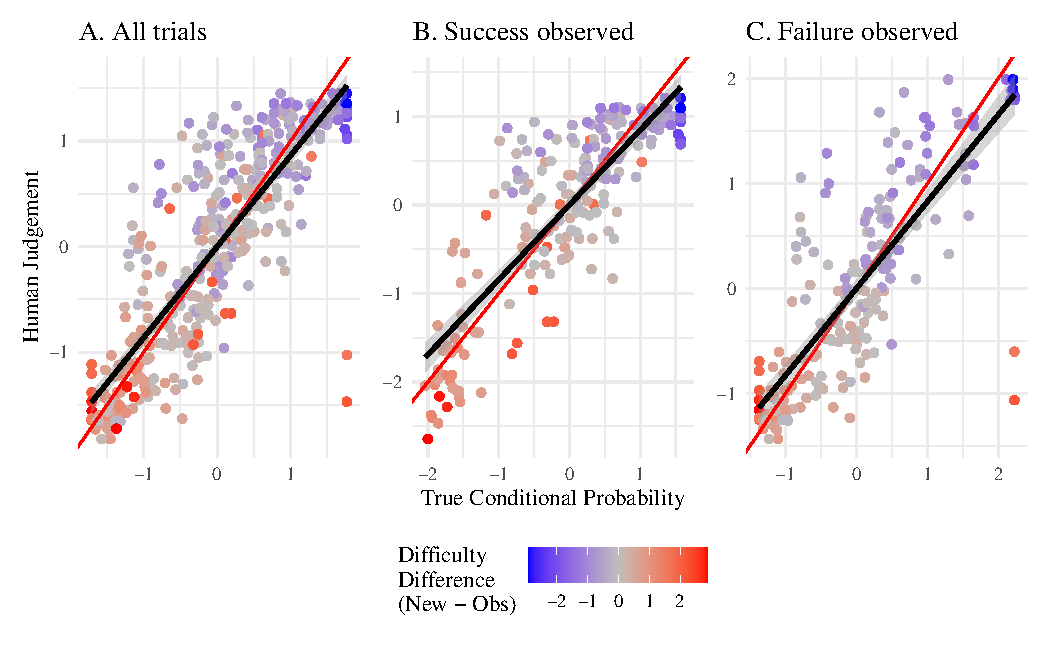
\includegraphics[keepaspectratio]{figures/S1-fig-behav-2-1.pdf}}
\caption{\label{fig:S1-fig-behav-2}Estimated Conditional Probability versus True Conditional Probability. Each data point is a pair of two questions.The red line represents the optimal prediction while the dark line represents the fit of the linear models.}
\end{figure}

We finally investigated how the models compared when we allowed to the parameters to differ for each individual rather than fixing them across all individuals. We did this because individuals may have different prior distributions of competence in the population. They may also have different priors about the role of luck in answering the questions. We therefore tested whether the main model fit individual level data better than heuristic model 1 (\textbf{RQ2}) and heuristic model 2 (\textbf{RQ3}). We used a maximum likelihood optimization to estimate the best free parameters for each participant. On average, our main model explained the behaviour of participants significantly better than Heuristic 1 (\(BIC_{Bayes}\) = 70.66 \(\pm\) 20.38; \(BIC_{Threshold}\) = 87.97 \(\pm\) 17.81; t(216) = -16.93, p \textless{} .001, paired t-test) and Heuristic 2 (\(BIC_{Anchor}\) = 80.86 \(\pm\) 19.8; t(216) = -10.84, p \textless{} .001, paired t-test). The Bayesian model was the best model for 72\% of participants whereas the Heuristic 1 accounted for 6\% and the Heuristic 2 accounted for 21\%.

\subsection{Exploring Response Time Data}\label{exploring-response-time-data}

We began by testing, for any pair of participants who got the same question correct (for all questions), in what proportion of these pairs the one who answered faster achieved a higher total score. For each pair, we identified which participant responded faster and then compared their total scores across the task. Pairs with identical response times were excluded (only 0.072\% of the pairs). We then calculated the proportion of pairs in which (a) the faster participant achieved a higher total score, (b) both participants achieved the same total score, and (c) the faster participant achieved a lower total score. We found that in 52.5\% of the pairs, the participant who got the right answer faster had a higher total score, in 10.2\% of the pairs participants tied, and in 37.3\% of pairs the participant who reached the correct answer faster had a lower total score.

In order to further investigate whether participants who were faster than their peers on a question they solved tended to be more accurate on other questions, we constructed a model which used participants' relative (scaled) speed on any particular question to predict accuracy on all other questions. We first defined an anchor question \emph{q} for each participant as any question they answered correctly. For each such \emph{q}, we computed that participant's relative speed on \emph{q} by z-scoring the negative response time within that question among the subset who were correct on \emph{q} (so higher values mean faster than peers who also solved \emph{q}). We then created, for every participant--anchor pair (id, \emph{q}), one row for each other target question \emph{r} \(\neq\) \emph{q}, with the binary outcome being whether the participant was correct on \emph{r}. From this dataset we fit a mixed-effects logistic regression predicting success on \emph{r} with a fixed effect for relative speed on \emph{q} and random effects for participant, \emph{r}, and \emph{q}.

We found that the fixed effect for relative speed on anchor question \emph{q} was very small and not significant (\(\beta\) = 0.0304, p = 0.193). Being faster than peers on a question a participant solved did not meaningfully predict accuracy on other questions.

Finally, we fit another mixed-effects logistic regression to investigate whether response time on a question predicted accuracy on that question across participants and items. Here we found that response time had a significant negative effect on accuracy (\(\beta\) = -0.104, p \textless{} .001), indicating that longer response times were associated with lower accuracy. Converting from log-odds, each one-second increase in response time corresponded to a 9.88\% decrease in the odds of answering correctly.

\section{Study 2}\label{study-2}

\subsection{Confirmatory Analyses}\label{confirmatory-analyses}

We first tested if participants were able to assess the difficulty of correctly answering the observed questions. We collected judgement of difficulty on the quiz 2 questions only as quiz 1 were materials from the first study. The analysis is not subdivided by time condition: both in the judgement phase and in the questionnaire phase, participants were presented with each condition half the time. A linear mixed effect model with random slope and intercept for participants showed that participants' estimations correctly tracked the difficulty of answering each question (H1: \(\beta\) = 0.39, t(313.06) = 16.85, p \textless{} .001).

To determine if the time condition in Quiz 2 provided information about the probability of answering correctly a question of the Quiz 1, we created pairs of Quiz 1 and Quiz 2 questions (e.g Q1.1-Q2.1, Q1.1-Q.2.2, etc.) from participants' answers. Note that this mirror the structure of the judgement phase: while H2a and H2b test if the time condition provide information (for correct and incorrect questions respectively), H4a and H4b test if participants rely on the time condition when making a judgement. We ran two logits mixed-effect models: one among participants who answered a given Quiz 2 question correctly and one among those who answered it incorrectly. In both models, the dependent variable was a binary variable coding if the question from Q1 was correctly answered and the independent variable was a factor coding if the Q2 question was solved (H2a) or failed (H2b) under the Fast or the Slow condition. We controlled for the specific pair with a random effect (therefore comparing for the same pair, the effect of solving/failing under the fast condition compared to the slow), the model also include random intercepts for participants. H2a was restricted to trials where the Q2 question was solved and H2b was restricted to trials where the Q2 question was failed. We found that for a given pair of Quiz 1 and Quiz 2 questions, among participants who correctly answered the Quiz 2 question, those who answered under a 20-second time limit have a higher chance of answering the Quiz 1 question than those who answered under a 40-second time limit (H2a: b = 0.51, z = 2.15, p = 0.031). Among participants who failed the Quiz 2 question, those who failed under a 20-second time limit also had a higher chance of answering the Quiz 1 question compared to those who failed under a 40-second time limit (H2b: b = 0.71, z = 2.63, p = 0.009). This indicate that, no matters the outcome on the Quiz 2 question, participants should attribute higher chance of success to participants in the Fast condition, although the effect is relatively small.\\

We replicated the analysis of study 1 and found that, on average, participants' predictions of the probabilities of success on different evaluated questions, given success or failure within the 20 second or 40 second time limit on an observed question, are significantly correlated with true conditional probabilities (H3: \(\beta\) = 0.89, t(98) = 19.47, p \textless{} .001, Adjusted \(R^2\) = 0.79). Mirroring the analyses of H2a and H2b, we tested if participants took into account the information provided by the time condition when predicting success/failure on evaluated Quiz 1 questions. Similar models than H2a and H2b were estimated, but with participants' binary predictions as the dependent variable and the observed time condition as the independent variable (still controlling for the pair presented and restricting the analyses among success/failure observed). Results show that participants do not take into account the information provided by the time condition when observing a correct answer under 20 second compared to 40 second (H4a: b = 0.17, z = 1.53, p = 0.125) or when observing an incorrect answer (H4b: b = 0.15, z = 1.62, p = 0.104).

We further tested if our results for H1 and H3 were robust when testing predictions of participants with minimal arithmetic ability (defined as the bottom 30\% score in the questionnaire). Participants with minimal arithmetic ability can both accurately predict the difficulty of each question (H1m: \(\beta\) = 0.32, t(88.04) = 8.16, p \textless{} .001) and predict the conditional probabilities of success on evaluated questions (H3m: \(\beta\) = 0.88, t(98) = 18.73, p \textless{} .001, Adjusted \(R^2\) = 0.78).

Moreover, participants' predictions of the conditional probabilities of success were still correlated with the true probability when analyzed at the trial level (H3i: b = 1.95, z = 46.19, p \textless{} .001).

\printbibliography

\end{document}
